%%%%%%%%%%%%%%%%%%%%%%%%%%%%%%%%%%%%%%%%%
% Beamer Presentation
% LaTeX Template
% Version 1.0 (10/11/12)
%
% This template has been downloaded from:
% http://www.LaTeXTemplates.com
%
% License:
% CC BY-NC-SA 3.0 (http://creativecommons.org/licenses/by-nc-sa/3.0/)
%
%%%%%%%%%%%%%%%%%%%%%%%%%%%%%%%%%%%%%%%%%

%----------------------------------------------------------------------------------------
%	PACKAGES AND THEMES
%----------------------------------------------------------------------------------------

\documentclass[aspectratio=169]{beamer}
\usepackage[utf8]{inputenc}
\usepackage{booktabs}
\usepackage{graphicx}
\usepackage{array}
\usepackage{caption}
\usepackage{threeparttable}
\usepackage{lscape}
\usepackage{import}
\usepackage{multirow, array}
\usepackage{amsmath}
\usepackage{csvsimple}
\usepackage{siunitx}
\usepackage{subfigure}
\usepackage{filecontents}
\newenvironment{wideitemize}{\itemize\addtolength{\itemsep}{10pt}}{\enditemize}
\usepackage{appendixnumberbeamer}
\usepackage{float}
\usepackage{amsmath}  
\usepackage{tikz,pgfplots}
\usepackage{tkz-fct}
\usepackage{hyperref}
\hypersetup{
    colorlinks=true,
    linkcolor=blue,
    filecolor=magenta,      
    urlcolor=cyan,
    pdftitle={Overleaf Example},
    pdfpagemode=FullScreen,
    }

\urlstyle{same}
\usepackage{amsthm}
\pgfplotsset{compat=1.10}
\usepgfplotslibrary{fillbetween}
\newcommand{\vertLineFromPoint}[1]{
  \draw[dashed] 
  (#1) -- (#1|-{rel axis cs:0,0})
}
\newcommand{\horLineFromPoint}[1]{
  \draw[dashed] 
  (#1) -- (#1-|{rel axis cs:0,0})
}
\mode<presentation> {
\AtBeginSection[]
{
    \begin{frame}
        \frametitle{Table of Contents}
        \tableofcontents[currentsection]
    \end{frame}
}

% The Beamer class comes with a number of default slide themes
% which change the colors and layouts of slides. Below this is a list
% of all the themes, uncomment each in turn to see what they look like.

%\usetheme{default}
%\usetheme{AnnArbor}
%\usetheme{Antibes} -
%\usetheme{Bergen}
%\usetheme{Berkeley}
%\usetheme{Berlin}
\usetheme{Boadilla}
%\usetheme{CambridgeUS}
%\usetheme{Copenhagen} -
%\usetheme{Darmstadt}
%\usetheme{Dresden}
%\usetheme{Frankfurt}
%\usetheme{Goettingen}
%\usetheme{Hannover}
%\usetheme{Ilmenau}
%\usetheme{JuanLesPins}
%\usetheme{Luebeck}
%\usetheme{Madrid}
%\usetheme{Malmoe}
%\usetheme{Marburg}
%\usetheme{Montpellier}
%\usetheme{PaloAlto}
%\usetheme{Pittsburgh}
%\usetheme{Rochester} -
%\usetheme{Singapore}
%\usetheme{Szeged}
%\usetheme{Warsaw}

% As well as themes, the Beamer class has a number of color themes
% for any slide theme. Uncomment each of these in turn to see how it
% changes the colors of your current slide theme.

%\usecolortheme{albatross}
%\usecolortheme{beaver}
%\usecolortheme{beetle}
%\usecolortheme{crane}
%\usecolortheme{dolphin}
%\usecolortheme{dove}
%\usecolortheme{fly}
%\usecolortheme{lily}
%\usecolortheme{orchid}
%\usecolortheme{rose}
%\usecolortheme{seagull}
%\usecolortheme{seahorse}
%\usecolortheme{whale}
%\usecolortheme{wolverine}

%\setbeamertemplate{footline} % To remove the footer line in all slides uncomment this line
\setbeamertemplate{footline}[frame number] % To replace the footer line in all slides with a simple slide count uncomment this line
\setbeamertemplate{theorems}[numbered]
\setbeamertemplate{navigation symbols}{} % To remove the navigation symbols from the bottom of all slides uncomment this line
}
\setbeamertemplate{caption}{\raggedright\insertcaption\par}
  \setbeamertemplate{enumerate items}[default]
\usepackage{graphicx} % Allows including images
\usepackage{booktabs} % Allows the use of \toprule, \midrule and \bottomrule in tables
%\usepackage {tikz}
\newtheorem*{theorem*}{Theorem}
\newtheorem*{lemma*}{Lemma}
\newtheorem*{proposition}{Proposition}
\newtheorem*{corollary*}{Corollary}
\newtheorem*{definition*}{Definition}
\DeclareMathOperator*{\argmin}{arg\,min}
\newtheorem*{assumption}{Assumption}
\usetikzlibrary {positioning}
% macro for inputting terminal nodes
\newcommand\term[2]{\node[below]at(#1){$#2$};}
%
%\usepackage {xcolor}

%----------------------------------------------------------------------------------------
%	TITLE PAGE
%----------------------------------------------------------------------------------------

\title[Obamacare]{Lecture 10: Understanding Obamacare and the Individual Mandate} % The short title appears at the bottom of every slide, the full title is only on the title page

\author{Jacob Kohlhepp} % Your name
\institute[UCLA] % Your institution as it will appear on the bottom of every slide, may be shorthand to save space
{
Econ 101 \\ % Your institution for the title page
\medskip
}
\date{\today} % Date, can be changed to a custom date

\begin{document}

\begin{frame}
\titlepage % Print the title page as the first slide
\end{frame}

\begin{frame}{Introduction}
\begin{wideitemize}
    \item We will use the tools we covered in the last lecture to think about the design of the Affordable Care Act (nickname: Obamacare)
    \item Everyone has opinions about politics (including me).
    \item The goal of this lecture is to think about the theory behind the bill.
    \item At the end we will have an open discussion about the theory and the pros/cons.
    \item I hope this lecture shows you how the ideas of this class have profound impacts on policy and your everyday life.
\end{wideitemize}
\end{frame}
\section{Background on the Affordable Care Act}
\begin{frame}{History of US Health Insurance}
    \begin{wideitemize}
        \item Since the Civil War, a very early form of insurance existed in the form is sickness funds.
        \item 1929: Great Depression put financial pressure on hospitals. 
        \item To accommodate, Baylor and then the American Hospital Association developed plans where people paid a premium out of their paycheck for a guarantee of 21 days in a hospital.
        \item WW2 wage controls + tax code changes + organized labor resulted in a dobling of Americans covered from 1940 to 1950.
        \item Further growth driven by Medicare and Medicaid expansions in the 1960s.
    \end{wideitemize}
\end{frame}

\begin{frame}{History of US Health Insurance}
    \begin{wideitemize}
        \item The rise of commercial insurance companies in the 60s and 70s drove competition for customers, and also drove adverse selection (why?)
        \item Blue Cross and Blue Shield moved away from a single premium price (why?)
        \item Since the 70s, many changes, including:
        \begin{wideitemize}
            \item Rise of managed care (HMOs, Kaiser, etc).
            \item Rise of PPOs (now 56\% of market).
            \item Rise of high deductible health plans (who might like these?)
            \item Increase in state regulations.
        \end{wideitemize}
        \item In 2010, the Affordable Care Act passed and changed many aspects.
    \end{wideitemize}
    Source: \hyperlink{https://account.ache.org/iweb/upload/Morrisey2253_Chapter_1-3b5f4e08.pdf}{History of Health Inusrance In the United States}
\end{frame}



\begin{frame}{Main Aspects of the ACA}
    \begin{wideitemize}
        \item \textbf{The Individual Mandate:} Those without health insurance must pay a tax penalty.
        \item \textbf{Employer Mandate:} Employers with 50 or more employees must offer health insurance coverage.
        \item \textbf{Medicaid Expansion:} Increase income limit for Medicaid eligibility.
        \item \textbf{American Health Benefit Exchanges:} Create exchanges for individuals to buy coverage. Implement subsidies and credits for low-income individuals using exchanges.
        \item \textbf{Cost Reductions:} Changes to prescription drug approval and other aspects to reduce costs.
        \item \textbf{Insurance Plan Regulations:} See Next Page
    \end{wideitemize}
\end{frame}


\begin{frame}{ACA Insurance Plan Regulations}
\begin{wideitemize}
    \item Must cover dependents until age 26.
    \item Premium increases must be reviewed by regulators.
    \item Limit premium differences based on age (must be less than 4:1)
    \item Prohibit lifetime limits on the dollar value of coverage
    \item Prohibit the exclusion of individuals with pre-existing conditions.
    \item Limit deductible prices
    
\end{wideitemize}

Source: \hyperlink{https://www.kff.org/health-reform/fact-sheet/summary-of-the-affordable-care-act/}{Kaiser Family Foundation Summary of the Affordable Care Act}

\end{frame}
\begin{frame}{Main Criticisms of the Bill}
    \begin{wideitemize}
        \item More access/lower prices will drive up demand and costs.
        \item Greater bureaucracy.
        \item Reducing consumer choice through the mandate.
        \item Disruption of existing coverage.
        \item Excessive burden on businesses (employer mandate).
        \item More taxes (tax on high value health insurance plans).
    \end{wideitemize}
\end{frame}




\section{Some Theory: Hidden Action and Moral Hazard}

\begin{frame}{The Two Channels}
There are two market failures that plague most insurance markets, including health insurance.
    \begin{wideitemize}
        \item \textbf{Adverse selection:} Less healthy people are more likely to buy health insurance if insurance companies cannot condition premiums on health status.
        \begin{wideitemize}
            \item Problem 2 from the problem set. Similar to Market for Lemons.
            \item People are also likely to wait to get insurance until they need it (this has been recognized as a big issue after the ACA passed) or to get high deductible plans.
            \item The result is that the pool of people that are insured will be on average less healthy than the overall population.
            \item This can greatly reduce insurance company profits.
        \end{wideitemize}
        \item \textbf{Moral Hazard:} Once people buy health insurance, they are likely to over utilize medical care because they only bear some of the marginal cost.
        \begin{wideitemize}
            \item Problem 1 from the problem set. Similar to manager and shareholder.
            \item Results in inefficiently high medical care spending.
        \end{wideitemize}
    \end{wideitemize}
\end{frame}

\begin{frame}{How Big Was Each Channel Pre-ACA?}

\centering

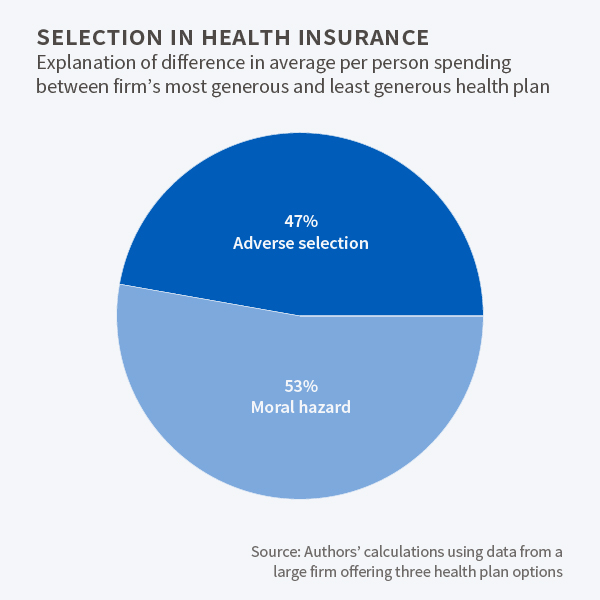
\includegraphics[width=0.45\textwidth]{health.jpg}

Source: Powell and Goldman (2020), Pre-ACA data
    
\end{frame}

\begin{frame}{How did the ACA Impact the Two Channels?}

\begin{wideitemize}
    \item Increased preventative care but increased risky drinking (Courtemanche et. al., 2019)
    \item Increased self-assessed health and risky drinking among young adults, but not preventative care (Barbaresco, 2015)
    \item Increased coverage for young people (Wettstein, 2017)
    \item Premiums rose from 2015 to 2016 (Graetz et. al., 2017)
    \item Individual mandate reduced adverse selection in MA. (Hackman et. al., 2015)
    \item \hyperlink{https://www.aeaweb.org/articles?id=10.1257/app.20170117}{Adverse Selection in ACA Exchange Markets: Evidence from Colorado (Panhans, 2019)}
\begin{wideitemize}
        \item A \$1 increase in premiums results in \$0.85-0.95 increase in healthcare expenditures in the ACA exchanges.
    \item A drop in premiums in Colorado resulted in \$1,324 in costs. 
    \item Many insurers are exiting the exchanges or raising premiums.
\end{wideitemize}
\end{wideitemize}

\end{frame}
\section{Discussion}

\begin{frame}{Questions}

\begin{wideitemize}
    \item Which criticisms of the ACA seem legitimate? Which do not?
    \item Given what has happened since passage, do you think the ACA will continue to achieve its goals?
    \item Was the ACA a good idea compared to the status quo?
    \item Do you have any alternatives? If so, what are the potential strengths and weaknesses of your approach.
    
    \item Open comments/debate are welcome. This is a controversial topic with no easy answers.
\end{wideitemize}
    
\end{frame}
\end{document}

